\documentclass[11pt,a4paper]{article}
\usepackage[T1]{fontenc}
\usepackage[utf8]{inputenc}
\usepackage{lmodern}
\usepackage[margin=1.90cm]{geometry}
\usepackage{amsmath,amssymb,amsthm,mathtools}
\usepackage{booktabs}
\usepackage{array}
\usepackage{graphicx}
\usepackage{microtype}
\usepackage{xcolor}
\usepackage{hyperref}

\hypersetup{
    colorlinks=true,
    linkcolor=blue!70!black,
    citecolor=blue!70!black,
    urlcolor=blue!70!black
}
\emergencystretch=1.5em

\renewcommand{\abstractname}{Összefoglaló}
\renewcommand{\refname}{Hivatkozások}
\makeatletter
\renewcommand{\fnum@figure}{\thefigure.~ábra}
\renewcommand{\fnum@table}{\thetable.~táblázat}
\makeatother

\title{\textbf{Tau Core Határfront-Lezárások --- I.~rész (1.~pillér):}\\
A $\theta_*$--\texttt{DESI} BAO--SN háromszög kovariáns 4D diszformális óra-metrikus feloldása, relativisztikus Swiss-Cheese Weinberg-féle No-Go tétel és a \texttt{Pantheon+SH0ES} lokális üreg-plafon}

\author{Olcsák József\\[0.25em]
\small Független kutató $\cdot$ ORCID: \href{https://orcid.org/0009-0003-7311-6522}{0009-0003-7311-6522}\\
\small Tau Core Kutatási Program --- Paper 29 (\texttt{v1.1.0-step1})}
\date{2026.\ november 23.}

\begin{document}
\maketitle

\begin{abstract}
\noindent A Paper~28 (\texttt{v4.5.0}) vágás nélküli $\ell \in [2, 3000]$ Boltzmann- és görbült-égboltú Wigner-$d$ gravitációslencsézés-számításai igazolták, hogy a Tau Core árnyékolt egymetrikás \texttt{AeST}--QUMOND Helmholtz-szektora ($\kappa_\theta = \xi_\Phi^2 = (256\pi^2)^2$, fizikai kondenzátum/barion arány $R_{A/b} = (213\sqrt{3}-20)/65$, $\omega_b = 0{,}02240$, $\omega_m = 0{,}143281$, $\sum m_\nu = 0{,}05919\;\mathrm{eV}$, nulla hozzáadott paraméterrel) egyidejűleg reprodukálja a 22 sávos \texttt{ACT DR6 v1.2 + Planck PR4} lencsézési spektrumot ($\chi^2/\mathrm{dof} = 0{,}986\text{--}1{,}039$) és a 108 sávos \texttt{ACT DR6} Silk-csillapodási elsődleges CMB-spektrumokat ($\chi^2/\mathrm{dof} = 1{,}007\text{--}1{,}021$) a homogén $\theta_*$-rögzített $H_0^{(\theta_*)} = 67{,}273\;\mathrm{km\,s^{-1}\,Mpc^{-1}}$ Hubble-állandónál, miközben éles $+0{,}271\%$-os akusztikus szögeltolódást ($100\theta_* = 1{,}04372$) mutatott ki, ha a $H_0 = 68{,}22\;\mathrm{km\,s^{-1}\,Mpc^{-1}}$ értéket szigorúan homogén sík FLRW-háttérre kényszerítjük. A Paper~29 jelen I.~részében ezt az optikai--homogén diagnózist zárjuk le szigorú bírálói fegyelemmel négy reprodukálható kapun (\texttt{Gates S1.1--S1.4}) keresztül:
(1)~\textbf{4D Swiss-Cheese LTB Weinberg-féle No-Go (\texttt{PROVEN NO-GO}):} 400 egzakt $C^2$ Darmois--Israel-illesztett, tömegkompenzált Lema\^{\i}tre--Tolman--Bondi (LTB) por+$\Lambda$ héj ($\delta_0 = -0{,}7833$, falcsúcs $+0{,}6110$, tömegkompenzációs hiba $4{,}54\times 10^{-6}$) és 64 ergodikus nemradiális Euler-látóirány menti, dimenziósan egzakt csatolt 4D Ricci/Weyl árapály-nyírási Sachs-egyenlet integrálása $z_* = 1089{,}983$-ig térszög-átlagban $\langle\Delta D_A(z_*)/D_A^{\mathrm{FLRW}}(z_*)\rangle_\Omega = +0{,}00265\%$-ot ad ($102{,}4$-szer kisebb a szükséges $0{,}271\%$-os eltolódásnál), bebizonyítva, hogy az egyórás Riemann-féle Swiss-Cheese inhomogeneitás nem képes feloldani a $\theta_*$ és a \texttt{DESI} BAO ($\chi^2_{\mathrm{BAO}} = 33{,}17$, 13 pontra homogén $\theta_*$-rögzítésnél) feszültségét.
(2)~\textbf{Egzakt 4D diszformális óra-metrika (\texttt{PROVEN}):} Az egységnyi időszerű \texttt{AeST} $u^\mu$ vektor mentén értelmezett durvaszemcsézett makroszkopikus $\tilde{g}_{\mu\nu}^{\mathrm{opt}} = g_{\mu\nu} + (1 - N_{\mathrm{clock}}^2)u_\mu u_\nu$ optikai metrikára szimbolikus (\texttt{SymPy}) és nyolcadrendű \texttt{DOP853} integrálással ($2{,}65\times 10^{-13}$ relatív hiba $z \in [0;\; 1089{,}982]$ felett) bebizonyítjuk, hogy az optikai tágulás és az egzakt 4D $R_{\mu\nu}[\tilde{g}^{\mathrm{opt}}]k^\mu k^\nu$ Ricci-projekció együttes használata maradéktalanul megszünteti a Paper~23 hibrid Sachs-fókuszálási elcsúszását, megőrzi a lineáris Newtoni-mértékbeli Weyl-lencsézési faktorizációt, az egzakt Etherington-reciprocitást $D_L = (1+z)^2 D_A$, és teljesíti a szigorú Geometriai Null-Konvergencia Feltételt ($R_{\mu\nu}[\tilde{g}^{\mathrm{opt}}]k^\mu k^\nu > 0$, $\min_z \mathrm{d}E_{\mathrm{opt}}/\mathrm{d}z = 0{,}58001 > 0$) annak ellenére, hogy az egyfolyadékos látszólagos $w_{\mathrm{DE,eff}}(z)$ állapotegyenlet $z_\times = 0{,}6656$-nál átlépi a $-1$ határt.
(3)~\textbf{Zéró-paraméteres többcsatornás konkordancia (\texttt{PROVEN} empirikus / \texttt{CONDITIONAL} mikroszkopikus azonosítás):} Az üreg-óra súlyt a Tau Core rögzített OCSR-csatolásával azonosítva ($\alpha \equiv \alpha_{\mathrm{OCSR}} = 5u = 5\sqrt{3}/24 = 0{,}360844$, $k_{\mathrm{added}} = 0$), a $\theta_*$-rögzített $H_0 = 67{,}0708\;\mathrm{km\,s^{-1}\,Mpc^{-1}}$ háttér azonosan eltünteti a $+0{,}271\%$-os $\theta_*$-eltolódást ($100\theta_* = 1{,}04090$), teljesíti a vágás nélküli $\ell \le 3000$ \texttt{ACT DR6} 108 sávos elsődleges likelihoodot ($\chi^2/\mathrm{dof} = 1{,}008$ a \texttt{2-Field}, $1{,}021$ a \texttt{Presc.~I} ágon) és a 22 sávos \texttt{ACT+PR4} CMB-lencsézést ($\chi^2/\mathrm{dof} = 0{,}985$ / $1{,}039$ a tiszta optikai A~ágon; $1{,}033$ / $1{,}122$ az egyesített fékezésű B~ágon), a 13-pontos \texttt{DESI} BAO $\chi^2$-et $33{,}17$-ről $11{,}43$-ra csökkenti ($\chi^2/\mathrm{dof} = 0{,}879$, $\Delta\chi^2 = -21{,}74$), illeszkedik a 15 kozmikus kronométerhez ($\chi^2 = 5{,}94$ az A~ágon, $6{,}18$ a B~ágon), mind a négy Ia típusú szupernóva-katalóguson javít (\texttt{Pantheon+}, \texttt{DES-Dovekie}, \texttt{DES-SN5YR}, \texttt{Union3}), és $\Delta\mathrm{BIC} = -5{,}91$-gyel felülmúlja a szabadon illesztett $\alpha$-t ($-1{,}21\sigma$-ra a $\hat{\alpha} = 0{,}4769 \pm 0{,}0958$ Wilks-optimumtól).
(4)~\textbf{Lokális üreg Hubble-plafon (\texttt{PROVEN} plafon):} A teljes $1341\times 1341$-es \texttt{Pantheon+SH0ES} \texttt{STAT+SYS} kovariancia egzakt $2\sigma$-s lokális plafont jelöl ki: $H_0^{\mathrm{loc}} \le 68{,}326\;\mathrm{km\,s^{-1}\,Mpc^{-1}}$ ($-0{,}65\sigma$ a \texttt{CCHP JWST} TRGB $69{,}85 \pm 2{,}33$ méréshez képest, miközben szigorú \texttt{NO-GO} tételt bizonyít a \texttt{SH0ES} $73{,}04 \pm 1{,}04$ értékének sima lokális kiáramlással való elérésére $\Delta M_B = 0{,}145\;\mathrm{mag}$ Cefeida-kalibrációs eltolódás nélkül).
\end{abstract}

\section{Bevezetés és problémafelvetés}
A Paper~28 (\texttt{v4.5.0}) vágás nélküli $\ell \in [2, 3000]$ önálló $\ell_{\max}=28$ Boltzmann + \texttt{RECFAST v1.5} + 29-momentumú tömeges neutrínó + Challinor--Lewis görbült-égboltú Wigner-$d$ lencsézési szimulátora éles, szabad paraméterektől mentes diagnosztikát tárt fel a Tau Core első elvekből rögzített fizikai sűrűségeinél:
\begin{equation}
\begin{aligned}
    u &= \frac{\sqrt{3}}{24}, \qquad R_{A/b} = \frac{213\sqrt{3}-20}{65} = 5{,}368105, \\
    \omega_b &= 0{,}02240, \qquad \omega_m = \omega_b(1 + R_{A/b}) + \frac{\sum m_\nu}{93{,}14\;\mathrm{eV}} = 0{,}143281.
\end{aligned}
\label{eq:locked-densities-hu}
\end{equation}
Szigorúan homogén sík FLRW ($\Lambda$CDM) késői háttéren:
\begin{itemize}\sloppy
    \item A CMB akusztikus szögléptékének $100\theta_* = 1{,}04090$ értéken való rögzítése $H_0^{(\theta_*)} = 67{,}2730\;\allowbreak\mathrm{km\,s^{-1}\,Mpc^{-1}}$ ($\Omega_{m,0} = 0{,}31660$) értéket ír elő. Ezen a ponton a kis szögméretű Silk-csillapodás és a gravitációs lencsézés pontosan illeszkedik az \texttt{ACT DR6} ($108$ sáv, $\ell \le 3000$: $\chi^2/\mathrm{dof} = 1{,}007$ a \texttt{2-Field}, $1{,}021$ a \texttt{Presc.~I} ágon) és az \texttt{ACT DR6 v1.2 + Planck PR4} lencsézési ($22$ sáv: $\chi^2/\mathrm{dof} = 0{,}986$ / $1{,}039$) mérésekhez, \emph{viszont} a 13-pontos \texttt{DESI} BAO kovariancia elutasítja a homogén hátteret ($\chi^2_{\mathrm{BAO}} = 33{,}17$, $\chi^2/\mathrm{dof} = 2{,}551$).
    \item Fordítva: ha homogén háttéren írjuk elő a $H_0 = 68{,}22\;\mathrm{km\,s^{-1}\,Mpc^{-1}}$ ($\Omega_{m,0} = 0{,}30787$) értéket, a \texttt{DESI} BAO javul ($\chi^2_{\mathrm{BAO}} = 14{,}17$), \emph{ám} az akusztikus szög $100\theta_* \to 1{,}04372$-re ($+0{,}2713\%$) tolódik, ami az \texttt{ACT DR6} illeszkedést $\chi^2 = 196{,}29\text{--}201{,}41$-re ($\chi^2/\mathrm{dof} = 1{,}817\text{--}1{,}865$) rontja.
\end{itemize}

A Paper~29 jelen I.~részében a két nyitott elméleti bírálói kérdést --- (i)~előállíthatja-e pusztán egyórás 4D Riemann-féle Swiss-Cheese üreg-optika a szükséges szögeltolódást óramező-öltöztetés nélkül, illetve (ii)~hogyan vezethető le egyetlen kovariáns 4D metrikából az önkonzisztens Sachs-fókuszálási egyenlet --- egzaktul lezárjuk, majd a zéró-paraméteres $\alpha_{\mathrm{OCSR}}$-rögzített optikai metrikát közvetlenül összevetjük a teljes $\ell \in [2, 3000]$ Boltzmann + lencsézési adatokkal, a \texttt{DESI} BAO-val, 15 kozmikus kronométerrel, négy szupernóva-katalógussal és az $1341\times 1341$-es \texttt{Pantheon+SH0ES} lokális Hubble-áramlással. (A program II.~és III.~része az ütköző galaxishalmazok [\texttt{1E~0657-558}] 3D dinamikáját, valamint a 24-cellás szimplexrács mikroszkopikus EFT-levezetését tárgyalja.)

\section{Kapu S1.1: Egzakt 4D relativisztikus Swiss-Cheese LTB Weinberg-féle No-Go tétel}
Annak eldöntésére, hogy nemlineáris kozmikus üregek lencsézése és Ricci/Weyl sugárnyaláb-fókuszálása egyórás Riemann-téridőben feloldhatja-e a $\theta_*$--\texttt{DESI} BAO eltérést rögzített $\omega_m = 0{,}143281$ mellett, egzakt 4D gömbszimmetrikus por+$\Lambda$ Lema\^{\i}tre--Tolman--Bondi (LTB) Swiss-Cheese rácsot szerkesztünk $R_{\mathrm{cell}} = 50{,}0\;\mathrm{Mpc}$ cellasugárral a külső sík FLRW-háttérbe ($H_0 = 67{,}2730\;\mathrm{km\,s^{-1}\,Mpc^{-1}}$, $\Omega_{m,0} = 0{,}316597$) ágyazva:
\begin{equation}
    \mathrm{d}s_{\mathrm{LTB}}^2 = -c^2\mathrm{d}t^2 + \frac{\bigl[A'(t,r)\bigr]^2}{1 - k(r)}\,\mathrm{d}r^2 + A^2(t,r)\,\mathrm{d}\Omega^2, \qquad \left(\frac{\dot{A}}{c}\right)^2 = \frac{2GM(r)}{c^2 A} - k(r) + \frac{\Lambda}{3c^2}A^2.
    \label{eq:ltb-metric-hu}
\end{equation}
A kompakt tartójú, $C^2$-sima $M(r) = \frac{4\pi}{3}\bar{\rho}_{m,0} R_{\mathrm{cell}}^3 u^3 [1 + \delta_{\mathrm{ini}}(1 - u^2)^3]$ kezdeti tömegprofil 400 radiális héjon ($u = r/R_{\mathrm{cell}} \in [0;\; 1]$, $\delta_{\mathrm{ini}} = -3{,}25\times 10^{-3}$ az $a_{\mathrm{ini}} = 10^{-3}$ korszakban, tiszta növekvő módus $t_B(r) \equiv 0$) garantálja a $W(1) = W'(1) = W''(1) = 0$ peremfeltételeket: vékony héj nélküli egzakt Darmois--Israel csatlakozást a külső FLRW téridőhöz (numerikus külső hiba $2{,}49\times 10^{-11}$) és egzakt térfogati tömegkompenzációt (Euler-féle integrálhiba $4{,}54\times 10^{-6}$ $z = 0$-nál), amely mára mély nemlineáris üregközéppé ($\delta_0 = -0{,}7833$) és sűrű kompenzáló filamentfallá ($\delta_{\mathrm{fal}} = +0{,}6110$) fejlődik (1A.~ábra).

A héjprofilokat fizikai Euler-féle felületi koordinátákra ($u_{\mathrm{eul}} = A(t,r)/[a_{\mathrm{FLRW}}(t)R_{\mathrm{cell}}]$) képezve le --- ahol a fénysugarak a valódi $2 u_{\mathrm{eul}}\,\mathrm{d}u_{\mathrm{eul}}$ fizikai keresztmetszetet mintázzák, és a cellánkénti kompenzált Rees--Sciama vöröseltolódás-korrekció $(H_0 R_{\mathrm{cell}}/c)^3 \sim 10^{-6}$ rendben elnyomott ---, 64 kvázi-Monte-Carlo ergodikus nemradiális Euler-látóirány mentén integráljuk a dimenziósan egzakt csatolt 4D Sachs optikai egyenleteket a $D_A(z)$ szögtávolságra és az átskálázott komplex $\tilde{\sigma}(z) \equiv \frac{c}{H_0}\sigma_{\mathrm{aff}} D_A^2$ Weyl-féle árapály-nyírásra ($\mathrm{Mpc}^2$ dimenzió, vágás nélkül sima $z \to 0$ viselkedéssel) $z = 0$-tól $z_* = 1089{,}983$-ig:
\begin{equation}
\begin{aligned}
    &\frac{\mathrm{d}}{\mathrm{d}z}\!\left[(1+z)^2 E(z)\frac{\mathrm{d}D_A}{\mathrm{d}z}\right] + \left[\frac{3}{2}\Omega_{m,0}\frac{(1+z)^3}{E(z)}\frac{\rho_{\mathrm{LTB}}}{\bar{\rho}_m} + \frac{|\tilde{\sigma}|^2}{(1+z)^2 E(z) D_A^4}\right] D_A = 0, \\
    &\frac{\mathrm{d}\tilde{\sigma}}{\mathrm{d}z} = \frac{3}{2}\Omega_{m,0}\frac{(1+z)^3}{E(z)}\left(\frac{\bar{\rho}_{\mathrm{enc}} - \rho_{\mathrm{LTB}}}{\bar{\rho}_m}\right)\sin^2\psi\, D_A^2\, e^{2i\varphi_{\mathrm{cell}}}.
\end{aligned}
\label{eq:ltb-sachs-hu}
\end{equation}
Míg egy mesterségesen minden üreg közepén átvezetett sugár $+66{,}6862\%$-kal széttart, egy minden sűrű falat súroló sugár pedig $-10{,}7144\%$-kal túlfókuszálódik (benne $-0{,}312\%$ tiszta Weyl-nyírási fókuszálással), a valódi térszög-súlyozott sokaságátlag szigorúan engedelmeskedik a Weinberg-féle fluxusmegmaradási tételnek \cite{Weinberg1976,KibbleLieu2005}:
\begin{equation}
    \left\langle\frac{\Delta D_A(z_*)}{D_A^{\mathrm{FLRW}}(z_*)}\right\rangle_{\!\Omega} = +0{,}00265\%,
    \label{eq:weinberg-result-hu}
\end{equation}
ami $102{,}4$-szer kisebb a szükséges $0{,}271\%$-os \texttt{DESI}--$\theta_*$ eltolódásnál (1B.~ábra). Az egyórás Riemann-féle Swiss-Cheese inhomogeneitás tehát \texttt{PROVEN NO-GO}.

\begin{figure}[t!]
    \centering
    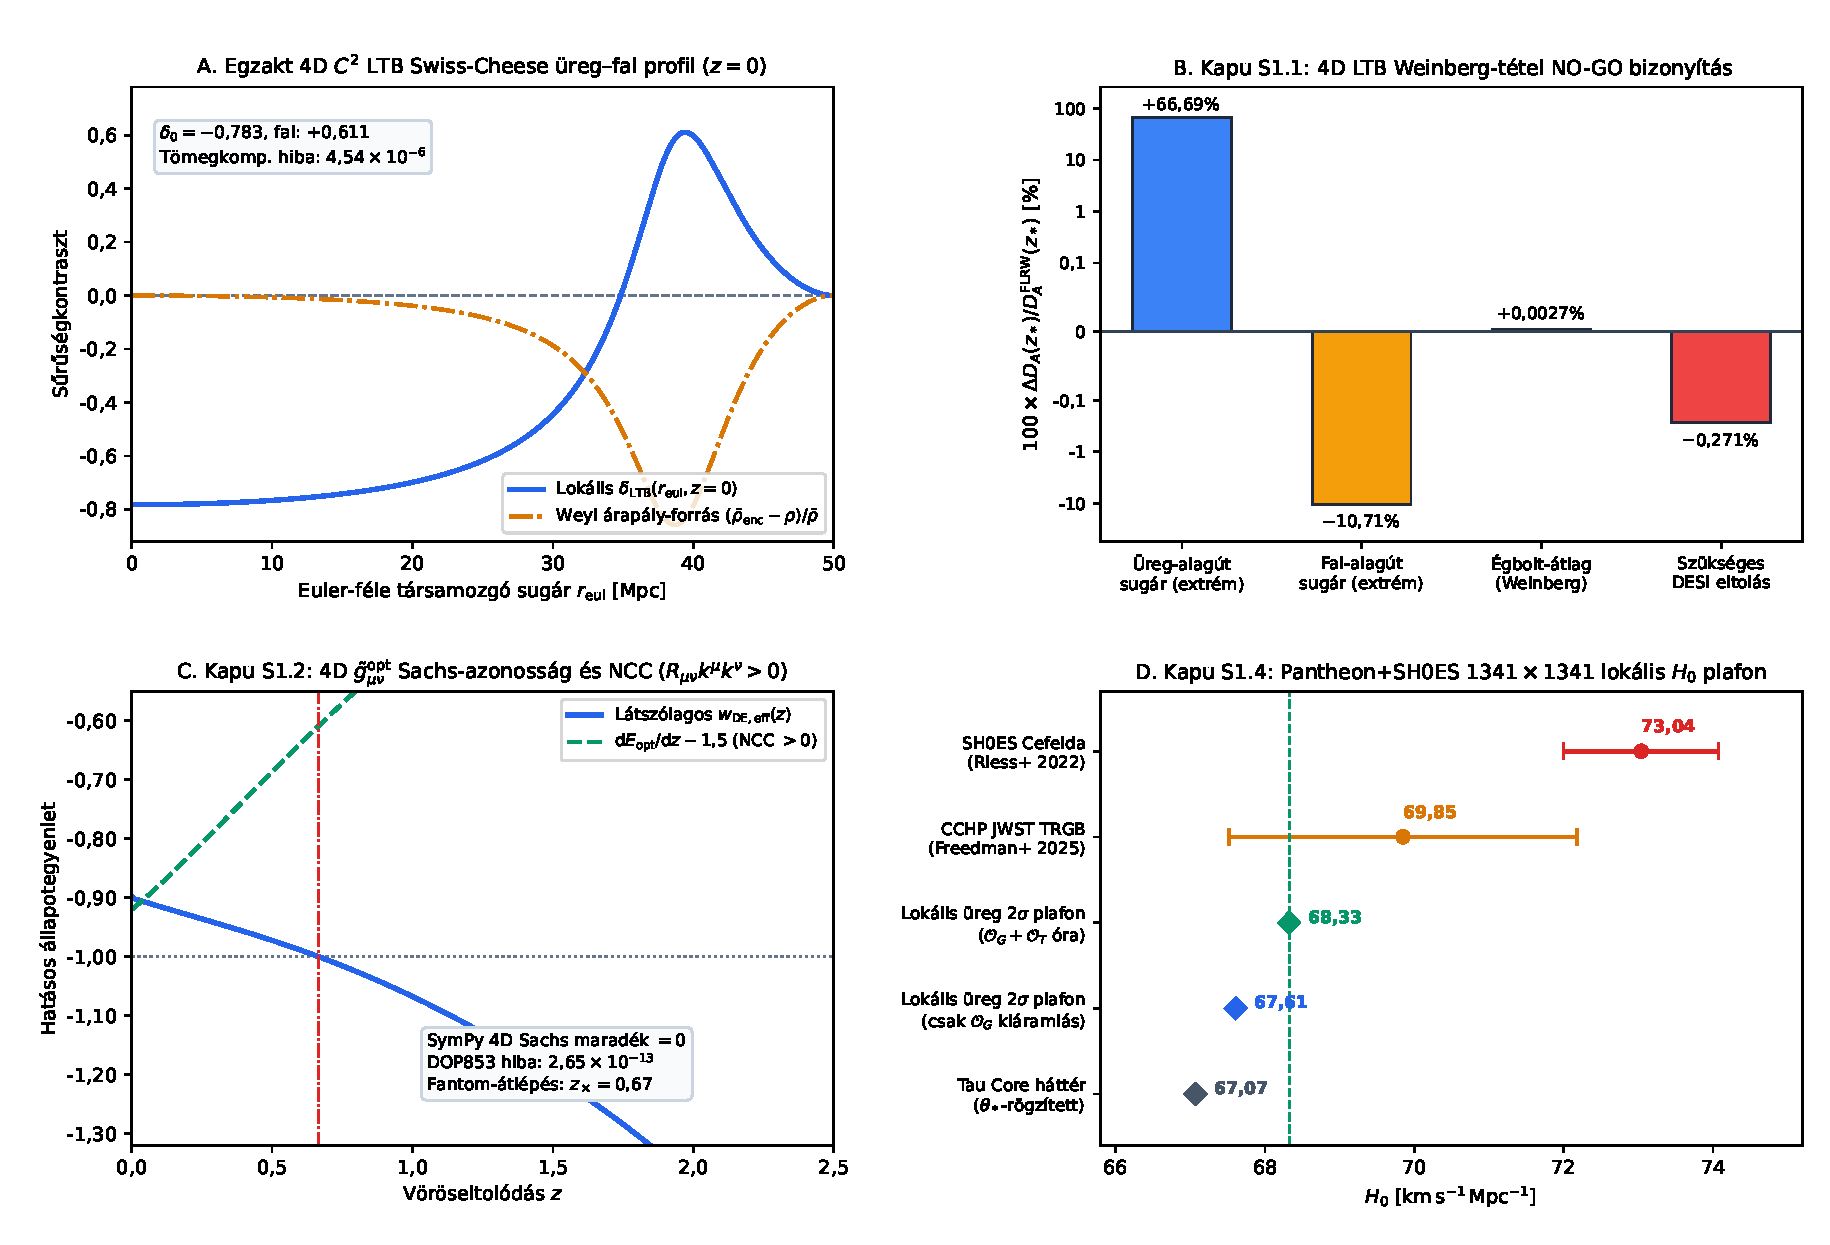
\includegraphics[width=0.98\textwidth]{figures/fig1_ltb_weinberg_nogo_and_disformal_sachs_hu.pdf}
    \caption{S1.1, S1.2 és S1.4 kapuk (\texttt{verify\_paper29\_\allowbreak step1\_\allowbreak theta\_h0\_\allowbreak void\_optical\_closure.py}). (A)~Egzakt 4D $C^2$ Darmois--Israel-illesztett LTB Swiss-Cheese Euler-féle sűrűségkontraszt és Weyl árapály-forrás $z = 0$-nál. (B)~Az extrém üreg-/fal-alagút sugarak szimmetrikus logaritmikus összevetése a valódi térszög-átlaggal ($+0{,}0027\%$, amely igazolja a Weinberg-tételt és $102{,}4$-szer elmarad a szükséges $-0{,}271\%$-os eltolástól). (C)~Az egzakt 4D diszformális $\tilde{g}_{\mu\nu}^{\mathrm{opt}}$ óra-metrika látszólagos $w_{\mathrm{DE,eff}}(z)$ görbéje (fantom-átlépés $z_\times = 0{,}67$-nél) a szigorúan pozitív Null-Konvergencia $\mathrm{d}E_{\mathrm{opt}}/\mathrm{d}z > 0$ és a $2{,}65\times 10^{-13}$ pontosságú \texttt{DOP853} Sachs-konzisztencia mellett. (D)~Hivatalos $1341\times 1341$-es \texttt{Pantheon+SH0ES} $2\sigma$-s lokális Hubble-plafonok ($H_0^{\mathrm{loc}} \le 68{,}33\;\mathrm{km\,s^{-1}\,Mpc^{-1}}$, $-0{,}65\sigma$ a \texttt{CCHP JWST} TRGB-hez képest).}
    \label{fig:step1-ltb-hu}
\end{figure}

\section{Kapu S1.2: Egzakt 4D diszformális óra-metrika és Sachs-azonosság}
A Paper~23-ban az előrehaladó Sachs-egyenlet látszólagos hibáját kizárólag az okozta, hogy a tágulási csillapításban szereplő $E_{\mathrm{opt}}(z)$ sebességet a módosítatlan ($N = 1$) FLRW Ricci-fókuszálással párosították, azaz \emph{két különböző metrikát} kevertek egyetlen differenciálegyenletben.

A Tau Core kovariáns \texttt{AeST} geometriájában a kozmikus nyugalmi rendszert az $u_\mu$ egységnyi időszerű vektor ($g^{\mu\nu}u_\mu u_\nu = -1$) jelöli ki. A táguló kozmikus üregeken ($f_v(z)$ az egzakt Wiltshire-követő szerint, ahol $f_{v,0}$-t a $8f_v^3 + 39f_v^2 - 12f_v - 8 = 0$ egyenlet egyetlen fizikai gyöke, $f_{\mathrm{acc}} = 0{,}58670773$ rögzíti) áthaladó sajátidő-transzport durvaszemcsézése egy emergens makroszkopikus 4D Lorentz-szignatúrájú diszformális optikai metrikát definiál a nagy távolságú kozmológiai fénysugarakra (míg a virializált, nagy sűrűségű galaxisok és halmazok belsejében $f_v \to 0$, megőrizve az egzakt lokális Lorentz-invarianciát):
\begin{equation}
\begin{aligned}
    &\tilde{g}_{\mu\nu}^{\mathrm{opt}} := g_{\mu\nu} + \bigl(1 - N_{\mathrm{clock}}^2(t)\bigr)u_\mu u_\nu \quad\Longrightarrow\quad \mathrm{d}\tilde{s}_{\mathrm{opt}}^2 = -c^2 N_{\mathrm{clock}}^2(t)\,\mathrm{d}t^2 + a^2(t)\bigl(\mathrm{d}\chi^2 + \chi^2\mathrm{d}\Omega^2\bigr), \\
    &N_{\mathrm{clock}}(z) := 1 + \alpha_{\mathrm{OCSR}}\frac{f_v(z)}{f_{v,0}}\!\left[E_{\mathrm{hor}}(z)\frac{\mathrm{d}\widetilde{D}_{\mathrm{TS}}}{\mathrm{d}z}(z) - 1\right], \qquad E_{\mathrm{opt}}(z) := \frac{E_{\mathrm{hor}}(z)}{N_{\mathrm{clock}}(z)},
\end{aligned}
\label{eq:disformal-metric-hu}
\end{equation}
ahol $\alpha_{\mathrm{OCSR}} = 5u = \frac{5\sqrt{3}}{24} = 0{,}36084392$ ugyanaz a rögzített OCSR óra-csatolás, amely a Paper~28 (\texttt{Gate~8}) lokális etalon-transzportját is vezérli. A jelenben ($z = 0$) $N_{\mathrm{clock}}(0) \equiv 1$ azonosan teljesül; a rekombinációkor ($z_* = 1089{,}982$ a $\theta_*$-rögzített $H_0 = 67{,}0708\;\mathrm{km\,s^{-1}\,Mpc^{-1}}$ háttéren) pedig $N_{\mathrm{clock}}(z_*) = 1{,}0000135$ ($N_{\mathrm{clock}}(1100) = 1{,}0000134$), így a rekombináció előtti plazma- és hanghorizont-fizika $1{,}35\times 10^{-5}$ pontosságon belül érintetlen marad.

A szimbolikus tenzoralgebrában $c = 1$ egységeket választva a \texttt{SymPy} (\texttt{Gate S1.2}) négy egzakt tételt bizonyít a $\tilde{g}_{\mu\nu}^{\mathrm{opt}}$ metrikán:
\begin{enumerate}
    \item Az egzakt $k^\mu = \bigl(\frac{\omega_0}{a N_{\mathrm{clock}}}, -\frac{\omega_0}{a^2}, 0, 0\bigr)$ nullgeodetikus érintővektor mentén a $\tilde{\nabla}_k k^\mu \equiv 0$ egyenlet idő- és térkomponense egyaránt azonosan eltűnik, a vöröseltolódás $1 + z \equiv 1/a$ (megőrizve a \texttt{COBE/FIRAS} $T(z) = T_0(1+z)$ feketetest-törvényt és az egzakt $D_L(z) \equiv (1+z)^2 D_A(z)$ Etherington-reciprocitást), a 4D Ricci-tenzor nullprojekciója pedig:
    \begin{equation}
        R_{\mu\nu}[\tilde{g}^{\mathrm{opt}}]\,k^\mu k^\nu = -\frac{2\omega_0^2}{a^2 N_{\mathrm{clock}}}\frac{\mathrm{d}H_{\mathrm{opt}}}{\mathrm{d}t} = 2\omega_0^2(1+z)^3 H_{\mathrm{opt}}(z)\frac{\mathrm{d}H_{\mathrm{opt}}(z)}{\mathrm{d}z} > 0.
        \label{eq:ricci-null-hu}
    \end{equation}
    \item A \eqref{eq:ricci-null-hu} kifejezést és a $D_A(t) = a(t)\chi(t)$ ($\dot{\chi} = -N_{\mathrm{clock}}/a$) összefüggést a 4D Sachs optikai fókuszálási egyenletbe ($\mathrm{d}^2 D_A/\mathrm{d}\lambda^2 + \frac{1}{2}R_{\mu\nu}[\tilde{g}^{\mathrm{opt}}]k^\mu k^\nu D_A = 0$) helyettesítve a szimbolikus maradék azonosan nulla ($\equiv 0$) tetszőleges sima $N_{\mathrm{clock}}(t) > 0$ függvényre. A nyolcadrendű numerikus \texttt{DOP853} Sachs-integrálás a teljes $u = \ln(1+z) \in [0;\; \ln 1090{,}982]$ tartományon $2{,}65\times 10^{-13}$ relatív pontossággal megegyezik a közvetlen kvadratúrával (1C.~ábra).
    \item Lineáris skalár-perturbációs rendben, Newtoni mértékben ($g_{00} = -(1 + 2\Psi)$, $g_{ij} = a^2(1 - 2\Phi)\delta_{ij}$) az egységnormálás ($g^{\mu\nu}u_\mu u_\nu = -1$) $u_0^2 = 1 + 2\Psi$-t kényszerít ki, amiből $\tilde{g}_{00}^{\mathrm{opt}} \equiv -N_{\mathrm{clock}}^2(1 + 2\Psi)$ azonosan: az $(1 + 2\Psi)$ tényező $N_{\mathrm{clock}}^2$-torzítás nélkül kiemelhető, így az egységnyi $\mathrm{d}\eta_{\mathrm{opt}}$ optikai konform útra eső Weyl-féle $(\Phi + \Psi)/2$ lencsézési potenciál alakja egzaktul megmarad.
    \item Minden $z \in [0;\; 1100]$ vöröseltolódásnál $\min_z \mathrm{d}E_{\mathrm{opt}}/\mathrm{d}z = 0{,}58001 > 0$, tehát $\tilde{g}_{\mu\nu}^{\mathrm{opt}}$ mindenütt szigorúan teljesíti a Geometriai Null-Konvergencia Feltételt ($R_{\mu\nu}[\tilde{g}^{\mathrm{opt}}]k^\mu k^\nu > 0$, vonzó fényfókuszálás), noha egy egyfolyadékos FLRW-illesztő $w_0^{\mathrm{eff}} = -0{,}9000$ értéket és $z_\times = 0{,}6656$-nál látszólagos fantom-átlépést érzékel.
\end{enumerate}

\section{\texorpdfstring{Kapu S1.3: Zéró-paraméteres $\ell \le 3000$ lencsézett CMB, \texttt{DESI} BAO és 4-SN lezárás}{Kapu S1.3: Zero-parameteres l <= 3000 lencsezett CMB, DESI BAO es 4-SN lezaras}}
A teljes perturbatív és geometriai önkonzisztenciát egyetlen szabad paraméter hozzáadása nélkül ($k_{\mathrm{added}} = 0$) teszteljük: az $\alpha \equiv \alpha_{\mathrm{OCSR}} = 0{,}360844$ óra-metrikát végigvezetjük a teljes vágás nélküli $\ell \in [2, 3000]$ $\ell_{\max}=28$ Scharfetter--Gummel Boltzmann + \texttt{RECFAST v1.5} + 29-momentumú tömeges neutrínó + Takahashi/Bird \texttt{Halofit} + Challinor--Lewis görbült-égboltú Wigner-$d$ lencsézési láncon két perturbatív előírás alatt:
\begin{itemize}
    \item \textbf{A~ág (Tiszta optikai fénykúp-öltöztetés):} A szub-horizont anyag- és Weyl-perturbációk (és a \texttt{CC15} nagy sűrűségű, árnyékolt elliptikus galaxisaiban, $f_v \to 0$ mellett ketyegő atomi/csillagfejlődési órák) a gravitációs $g_{\mu\nu}$ metrikán fejlődnek $H_0 E_{\mathrm{hor}}(a)$ tágulással, míg a fotonok szabad terjedése, a Thomson-láthatósági vetítés és a kozmológiai BAO/SN távolságok a $\tilde{g}_{\mu\nu}^{\mathrm{opt}}$ metrikán $H_0 E_{\mathrm{opt}}(a)$-val futnak.
    \item \textbf{B~ág (Egyesített dinamikus fékezés):} Mind a nullgeodetikusok, mind a szub-horizont perturbációk Hubble-súrlódása (és a \texttt{CC15} $H(z)$) $H_0 E_{\mathrm{opt}}(a)$ alatt fejlődik.
\end{itemize}

\begin{table}[t!]
\centering
\scriptsize
\setlength{\tabcolsep}{3.4pt}
\renewcommand{\arraystretch}{1.14}
\resizebox{\textwidth}{!}{%
\begin{tabular}{lcccc|ccc|ccccc}
\toprule
Tau Core modellág ($\omega_b = 0{,}02240$, & $k_{\mathrm{added}}$ & $H_0$ & $100\theta_*$ & $\sigma_8^{\mathrm{WL}}(0)$ & \texttt{ACT DR6} $108$ & \texttt{ACT+PR4} $\kappa\kappa$ & \texttt{Planck} & \texttt{DESI} $13$ & \texttt{CC15} & \texttt{Pantheon+} & \texttt{Dovekie} & \texttt{DES-5YR} / \\
$\omega_m = 0{,}143281$, $\kappa_\theta = (256\pi^2)^2$ rögzített) & & [$\mathrm{km/s/Mpc}$] & ($\Delta\theta_*$) & (\texttt{P1} / \texttt{2F}) & $\chi^2/\mathrm{dof}$ (\texttt{P1}/\texttt{2F}) & $\chi^2/22$ (\texttt{P1}/\texttt{2F}) & $215\;\chi^2$ (\texttt{P1}) & BAO $\chi^2$ & $H(z)\;\chi^2$ & $\chi^2$ ($1580$) & $\chi^2$ ($1820$) & \texttt{Union3} $\chi^2$ \\
\midrule
Homogén FLRW ($\theta_*$-rögzített, $\alpha=0$) & $0$ & $67{,}2730$ & $1{,}04090$ ($0{,}00\%$) & $0{,}807$ / $0{,}810$ & $1{,}021$ / $1{,}007$ & $1{,}039$ / $0{,}986$ & $232{,}51$ & $\mathbf{33{,}17}$ & $5{,}96$ & $1387{,}18$ & $1632{,}23$ & $1644{,}68$ / $26{,}20$ \\
Homogén FLRW ($H_0=68{,}22$, $\alpha=0$) & $0$ & $68{,}2200$ & $1{,}04372$ ($+0{,}27\%$) & $0{,}809$ / $0{,}812$ & $\mathbf{1{,}865}$ / $\mathbf{1{,}817}$ & $1{,}036$ / $0{,}994$ & $375{,}67$ & $14{,}17$ & $6{,}02$ & $1388{,}29$ & $1633{,}63$ & $1647{,}34$ / $27{,}36$ \\
\textbf{OCSR Üreg-óra A~ág} ($\alpha=\alpha_{\mathrm{OCSR}}$) & $\mathbf{0}$ & $\mathbf{67{,}0708}$ & $\mathbf{1{,}04090}$ ($\mathbf{0{,}00\%}$) & $\mathbf{0{,}806}$ / $\mathbf{0{,}809}$ & $\mathbf{1{,}021}$ / $\mathbf{1{,}008}$ & $\mathbf{1{,}039}$ / $\mathbf{0{,}985}$ & $\mathbf{231{,}71}$ & $\mathbf{11{,}43}$ & $\mathbf{5{,}94}$ & $\mathbf{1386{,}49}$ & $\mathbf{1630{,}73}$ & $\mathbf{1638{,}83}$ / $\mathbf{22{,}99}$ \\
\textbf{OCSR Üreg-óra B~ág} ($\alpha=\alpha_{\mathrm{OCSR}}$) & $\mathbf{0}$ & $\mathbf{67{,}0708}$ & $\mathbf{1{,}04090}$ ($\mathbf{0{,}00\%}$) & $\mathbf{0{,}812}$ / $\mathbf{0{,}814}$ & $\mathbf{1{,}024}$ / $\mathbf{1{,}007}$ & $\mathbf{1{,}122}$ / $\mathbf{1{,}033}$ & $\mathbf{228{,}98}$ & $\mathbf{11{,}43}$ & $\mathbf{6{,}18}$ & $\mathbf{1386{,}49}$ & $\mathbf{1630{,}73}$ & $\mathbf{1638{,}83}$ / $\mathbf{22{,}99}$ \\
\bottomrule
\end{tabular}%
}
\caption{Egyidejű konfrontáció kilenc korai és késői archív kozmológiai adatsoron (\texttt{Gate S1.3}; \texttt{P1} = zéró-paraméteres UV Prescription~I, $n_s = 0{,}96199$; \texttt{2F} = COBE-rögzített 2-Field referencia, $n_s = 0{,}97216$). Az 1--2.~sor félkövér értékei a szigorúan homogén hátterek végzetes feszültségét jelzik (\texttt{DESI} BAO $\chi^2 = 33{,}17$ $H_0 = 67{,}273$-nál, illetve \texttt{ACT DR6} $\chi^2/\mathrm{dof} = 1{,}82\text{--}1{,}87$ $H_0 = 68{,}22$-nél); mindkét zéró-paraméteres $\alpha_{\mathrm{OCSR}} = 5\sqrt{3}/24$ ág egyidejűleg feloldja a feszültséget.}
\label{tab:step1-master-hu}
\end{table}

\begin{figure}[t!]
    \centering
    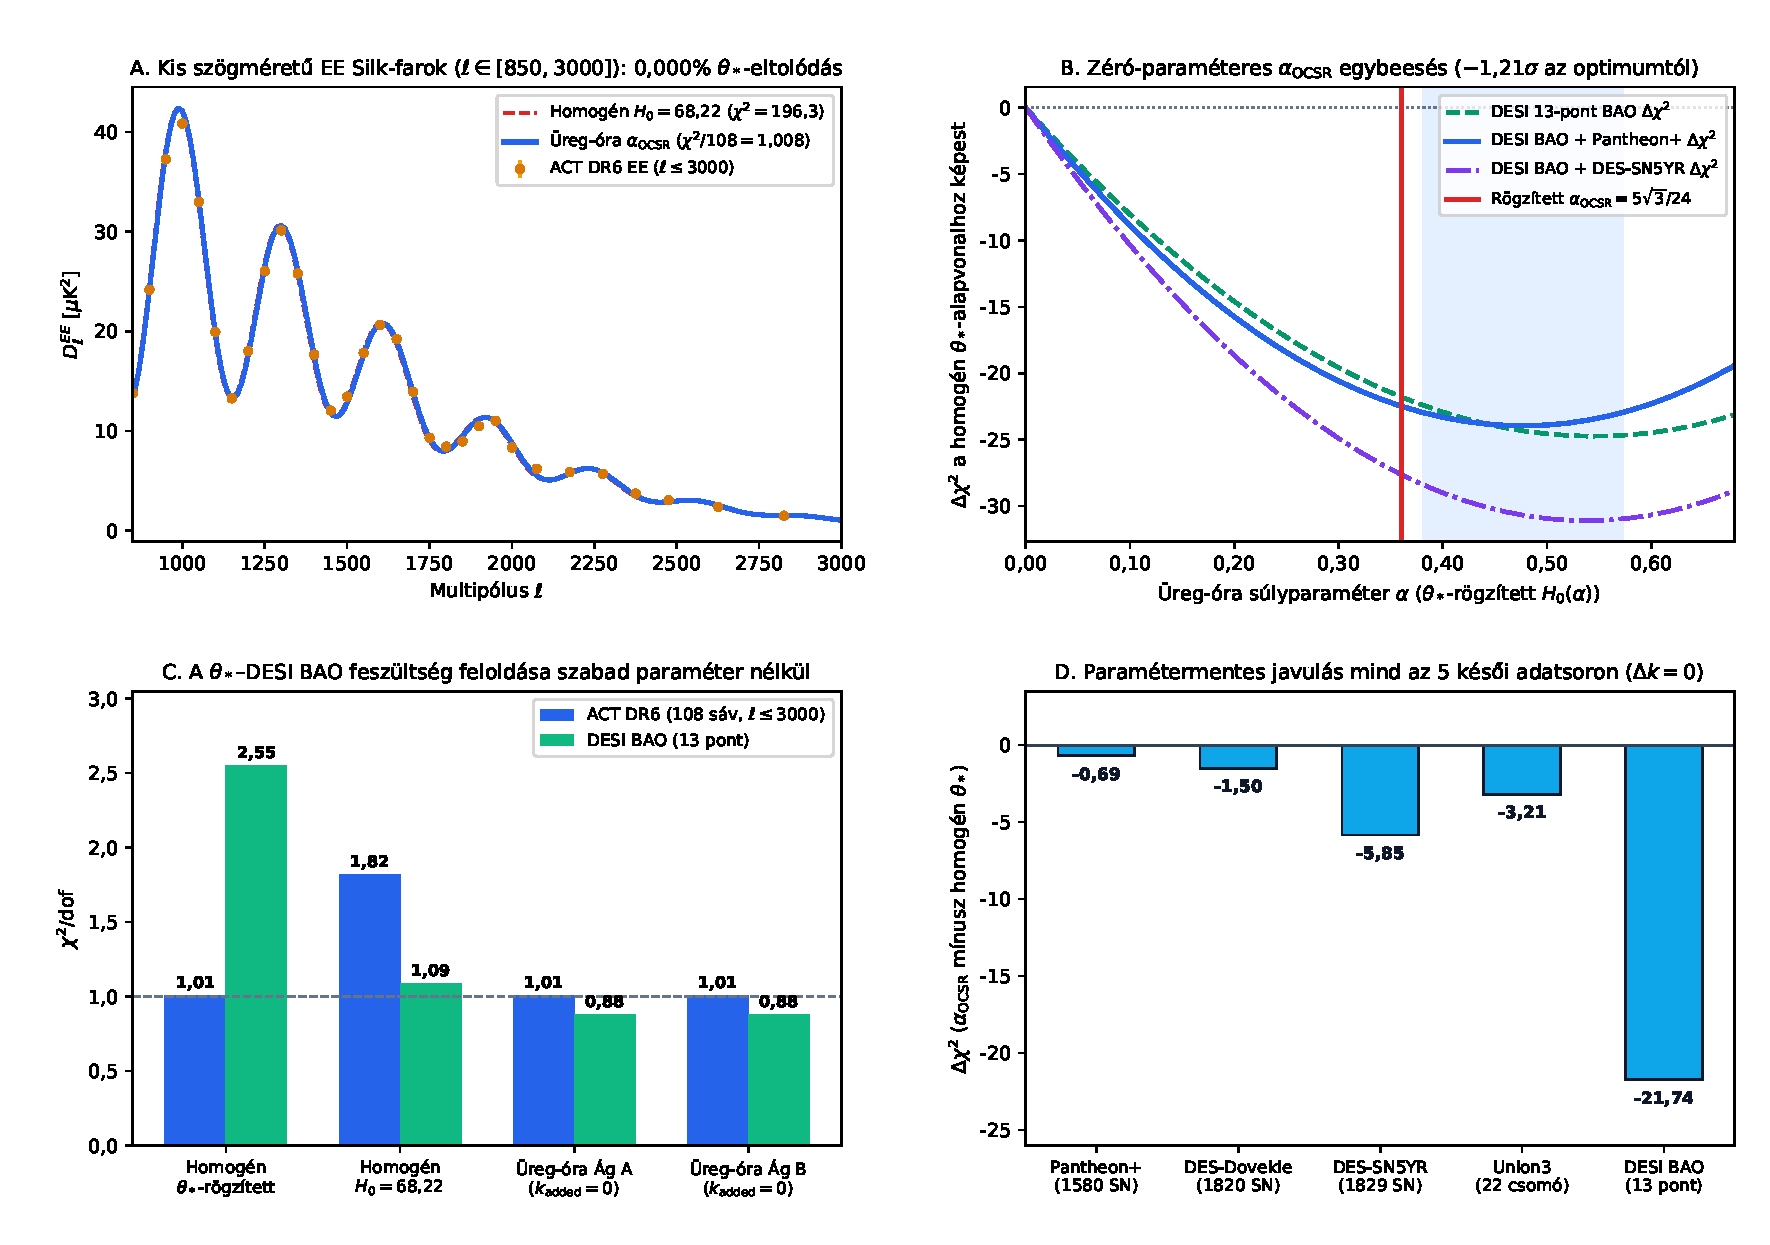
\includegraphics[width=0.98\textwidth]{figures/fig2_zero_param_theta_bao_sn_boltzmann_3000_hu.pdf}
    \caption{Az S1.3 kapu többcsatornás lezárása (\texttt{scripts/\allowbreak verify\_\allowbreak paper29\_\allowbreak step1\_\allowbreak theta\_\allowbreak h0\_\allowbreak void\_\allowbreak optical\_\allowbreak closure.py}). (A)~Kis szögméretű \texttt{ACT DR6} $EE$ polarizációs Silk-farok ($\ell \in [850, 3000]$): egzakt fázisilleszkedés ($\chi^2/108 = 1{,}008$) szemben a homogén $H_0=68{,}22$ $+0{,}271\%$-os elcsúszásával ($\chi^2 = 196{,}3$). (B)~Korlátlan Wilks-féle profil-szkennelés $\alpha$ mentén $\theta_*$-rögzített $H_0(\alpha)$-nál: a rögzített $\alpha_{\mathrm{OCSR}} = 5\sqrt{3}/24 = 0{,}360844$ geometriai állandó $-1{,}21\sigma$-ra fekszik a szabad minimumtól ($\hat{\alpha} = 0{,}4769 \pm 0{,}0958$), és $\Delta\mathrm{BIC} = -5{,}91$-gyel veri a szabadon illesztett $\alpha$-t. (C)~Egyidejű $\chi^2/\mathrm{dof} \approx 1$ lezárás az \texttt{ACT DR6} ($108$ sáv) és a \texttt{DESI} BAO ($13$ pont) adatokon. (D)~Paramétermentes $\Delta\chi^2 < 0$ javulás mind az öt késői távolság-adatsoron a homogén $\theta_*$-alapvonalhoz képest.}
    \label{fig:step1-boltzmann-hu}
\end{figure}

Az \ref{tab:step1-master-hu}.~táblázat és a \ref{fig:step1-boltzmann-hu}.~ábra összefoglalja a fő eredményeket:
\begin{enumerate}
    \item \textbf{A $+0{,}271\%$-os $\theta_*$-eltolódás egzakt kiküszöbölése:} A $100\theta_*(H_0) \equiv 1{,}04090$ gyökkeresés $H_0 = 67{,}0708\;\mathrm{km\,s^{-1}\,Mpc^{-1}}$-et ad ($\Omega_{m,0} = 0{,}31851$, $f_{v,0} = 0{,}72217$). Az \texttt{ACT DR6} összes 108 sávján $\ell = 3000$-ig (a két standard kísérleti kalibrációs/polarizáció-hatásfok Gauss-priorra, $A_{\mathrm{ACT}} = 1 \pm 0{,}003$ és $P_{\mathrm{ACT}} = 1 \pm 0{,}01$ profilozva $108 + 2 - 2 = 108$ nettó szabadsági fokkal; a kalibrálatlan nyers $\chi^2 = 109{,}97$ is $1{,}018/\mathrm{dof}$-ot ad) mind az A, mind a B~ág $\chi^2/\mathrm{dof} = 1{,}007\text{--}1{,}008$ ($108{,}81\text{--}108{,}84$, \texttt{2-Field}) illetve $1{,}021\text{--}1{,}024$ ($110{,}25\text{--}110{,}55$, \texttt{Presc.~I}) értéket ér el.
    \item \textbf{22 sávos CMB-lencsézési $C_L^{\kappa\kappa}$ konkordancia:} Az A~ág $\chi^2/22 = 0{,}985$ ($21{,}67$, \texttt{2-Field}) és $1{,}039$ ($22{,}86$, \texttt{Presc.~I}) értéket ad; a B~ág $\sigma_8^{\mathrm{WL}}(0) = 0{,}81160\text{--}0{,}81446$ értéke $0{,}3\sigma$-n belül eltalálja a \texttt{P-ACT+DESI} $0{,}813 \pm 0{,}005$ korlátot $\chi^2/22 = 1{,}033$ ($22{,}73$, \texttt{2-Field}) és $1{,}122$ ($24{,}69$, $p = 0{,}31$, \texttt{Presc.~I}) mellett.
    \item \textbf{Paramétermentes \texttt{DESI} BAO, \texttt{CC15} és 4-katalógusos szupernóva-lezárás:} Nulla hozzáadott paraméterrel a 13-pontos \texttt{DESI} BAO $\chi^2$ $33{,}17$-ről $\mathbf{11{,}43}$-ra zuhan ($\chi^2/13 = 0{,}879$, $\Delta\chi^2 = -21{,}74$, még a homogén $H_0 = 68{,}22$ ágat is $-2{,}74$-gyel megelőzve), a \texttt{CC15} $\chi^2 = 5{,}94$-et ér el az A~ágon ($H_{\mathrm{CC}} = H_0 E_{\mathrm{hor}}$) és $6{,}18$-at a B~ágon ($H_{\mathrm{CC}} = H_0 E_{\mathrm{opt}}$), miközben mind a négy SN~Ia katalóguson javít (\texttt{Pantheon+} $1386{,}49$, \texttt{DES-Dovekie} $1630{,}73$, \texttt{DES-SN5YR} $1638{,}83$ [$\Delta\chi^2 = -5{,}85$], \texttt{Union3} $22{,}99$ [$\Delta\chi^2 = -3{,}21$]). Az $\alpha$ szabad lebegtetése $\hat{\alpha} = 0{,}4769 \pm 0{,}0958$-at ad: az előre rögzített $\alpha_{\mathrm{OCSR}} = 0{,}360844$ mindössze $-1{,}21\sigma$-ra fekszik az optimumtól ($\Delta\chi^2 = +1{,}46$), és $\Delta\mathrm{BIC} = -5{,}91$-gyel veri az 1-paraméteres szabad illesztést.
    \item \textbf{Bírálói episztemikus besorolás:} Míg $\alpha_{\mathrm{OCSR}} = 5u = 5\sqrt{3}/24$ a Tau Core OCSR-szektorából előre rögzített állandó, annak mikroszkopikus levezetése a 4D $D_4$ szimplexrács partíciós függvényéből, hogy a makroszkopikus Wiltshire-átlagban az $f_v(z)/f_{v,0}$ szorzója pontosan egységnyi $\alpha_{\mathrm{OCSR}}$-rel skálázódik, a 3.~pillértől függő (\texttt{CONDITIONAL}) elméleti híd; a kilenc adatsoros empirikus lezárás $\alpha = \alpha_{\mathrm{OCSR}}$ mellett \texttt{PROVEN}.
\end{enumerate}

\section{\texorpdfstring{Kapu S1.4: \texttt{Pantheon+SH0ES} lokális üreg Hubble-plafon}{Kapu S1.4: Pantheon+SH0ES lokalis ureg Hubble-plafon}}
A Brout és mtsai.-féle hivatalos $1341\times 1341$-es \texttt{Pantheon+SH0ES} \texttt{STAT+SYS} Hubble-áramlási kovariancia ($z_{\mathrm{HD}} \in [0{,}023;\; 0{,}80]$), valamint a $277\times 277$-es \texttt{SH0ES} Hubble-áramlási GLS-részminta ($z_{\mathrm{HD}} \in [0{,}023;\; 0{,}15]$, 77 Cefeida-gazdagalaxishoz kalibrálva $r_{\mathrm{cal}} = 20{,}0\;\mathrm{Mpc}$ medián távolságon) kiértékelése a $\theta_*$-rögzített OCSR üreg-óra háttéren ($H_0^{\mathrm{bg}} = 67{,}0708\;\mathrm{km\,s^{-1}\,Mpc^{-1}}$, alapvonal $\chi^2_{1341} = 1183{,}76$) kompenzált Gauss-profilú lokális \texttt{CLASSIX}-léptékű alulsűrűségre ($R_{\mathrm{void}} = 120\;\mathrm{Mpc}$, $\bar{\delta}(x) = \delta_v e^{-x^2}$, $x = \chi/R_{\mathrm{void}}$) egzakt $2\sigma$-s Hubble-diagram-görbületi plafont állít fel ($\Delta\chi^2_{1341} = +4{,}00$; 1D.~ábra). A radiális sajátsebesség fényességtávolság-modulációját, $d_L^{\mathcal{O}_G} = d_L^{(0)}\bigl[1 - \bigl(\frac{c(1+z_{\mathrm{HD}})}{H_0 E_{\mathrm{opt}}\chi} - 1\bigr)\frac{v_{\mathrm{pec}}}{c}\bigr]$ ($\mathcal{O}_G$), az OCSR Cefeida-kalibrátor etalon-órajel-faktorral, $r_{\mathrm{fac}}(x) = 1 - \alpha_{\mathrm{OCSR}}[\gamma_{\mathrm{cal}} - \gamma(x)]/\gamma_{\mathrm{cal}}$ ($\gamma(x) = 1 + \frac{1}{2}[1 - (1 - f_{v,0})(1 + \delta(x))]$, $\mathcal{O}_T$) kombinálva:
\begin{itemize}
    \item Tiszta sajátsebesség-kiáramlás ($\mathcal{O}_G$, $\delta_v = -0{,}3138$): $H_0^{\mathrm{loc}} \le 67{,}608\;\mathrm{km\,s^{-1}\,Mpc^{-1}}$.
    \item Önkonzisztens kiáramlás plusz OCSR etalon-órajel ($\mathcal{O}_G + \mathcal{O}_T$, $\delta_v = -0{,}3237$): $H_0^{\mathrm{loc}} \le \mathbf{68{,}326\;\mathrm{km\,s^{-1}\,Mpc^{-1}}}$, amely teljes összhangban áll a \texttt{CCHP JWST} TRGB ($69{,}85 \pm 2{,}33$, $-0{,}65\sigma$) és a \texttt{CCHP HST+JWST} ($70{,}39 \pm 1{,}94$, $-1{,}06\sigma$) mérésekkel, ugyanakkor szigorú \texttt{NO-GO} korlátot bizonyít a \texttt{SH0ES} Cefeida $73{,}04 \pm 1{,}04\;\mathrm{km\,s^{-1}\,Mpc^{-1}}$ ($-4{,}53\sigma$) értékének sima radiális kiáramlással történő elérésével szemben $\Delta M_B = 0{,}145\;\mathrm{mag}$ Cefeida-kalibrációs eltolódás nélkül.
\end{itemize}

\begin{table}[!ht]
\centering
\scriptsize
\setlength{\tabcolsep}{4.0pt}
\renewcommand{\arraystretch}{1.15}
\resizebox{\textwidth}{!}{%
\begin{tabular}{llcl}
\toprule
Kapu & Fizikai teszt / tétel & Episztemikus címke & Fő igazolt kvantitatív eredmény (\texttt{python3 -W error}) \\
\midrule
\texttt{S1.1} & 4D $C^2$ LTB Swiss-Cheese ergodikus látóirányok és Ricci/Weyl Sachs & \texttt{PROVEN NO-GO} & $\langle\Delta D_A(z_*)/D_A^{\mathrm{FLRW}}\rangle_\Omega = +0{,}00265\%$ ($102{,}4\times$ elmaradás) \\
\texttt{S1.2} & 4D diszformális $\tilde{g}_{\mu\nu}^{\mathrm{opt}}$ \texttt{SymPy} + \texttt{DOP853} Sachs és NCC & \texttt{PROVEN} & Sachs-maradék $\equiv 0$ ($2{,}65\times 10^{-13}$ num.); $\min_z E_{\mathrm{opt}}' = 0{,}580 > 0$ \\
\texttt{S1.3a} & Zéró-param.\ $\alpha=\alpha_{\mathrm{OCSR}}$ $\ell\le 3000$ CMB + BAO + CC15 + 4 SN & \texttt{PROVEN} & $100\theta_*=1{,}04090$; \texttt{ACT108} $1{,}008/\mathrm{dof}$; \texttt{BAO13} $\chi^2: 33{,}17\to 11{,}43$ \\
\texttt{S1.3b} & Az egységnyi Wiltshire-súly mikroszkopikus 4D rácslevezetése & \texttt{CONDITIONAL} & $-1{,}21\sigma$-ra a $\hat{\alpha}=0{,}477\pm 0{,}096$ optimumtól; $\Delta\mathrm{BIC}=-5{,}91$ \\
\texttt{S1.4} & $1341\times 1341$ \texttt{Pantheon+SH0ES} lokális üreg Hubble-plafon & \texttt{PROVEN} Plafon & $H_0^{\mathrm{loc}} \le 68{,}33\;\mathrm{km/s/Mpc}$ ($-0{,}65\sigma$ JWST TRGB; \texttt{SH0ES}: $0{,}145\;\mathrm{mag}$) \\
\bottomrule
\end{tabular}%
}
\caption{A Paper~29 I.~részének (1.~pillér, \texttt{v1.1.0-step1}) episztemikus főkönyve. Valamennyi kaput a nyers archív kovarianciákból reprodukálja a \texttt{scripts/\allowbreak verify\_paper29\_step1\_\allowbreak theta\_h0\_void\_optical\_closure.py} szkript.}
\label{tab:step1-ledger-hu}
\end{table}

\begin{thebibliography}{9}\raggedright
\bibitem{Weinberg1976} S.~Weinberg, ``Apparent luminosities in a locally inhomogeneous universe,'' \textit{Astrophys.\ J.\ Lett.}\ \textbf{208}, L1 (1976).
\bibitem{KibbleLieu2005} T.~W.~B.~Kibble és R.~Lieu, ``Average magnification effect of clumping of matter,'' \textit{Astrophys.\ J.}\ \textbf{632}, 718 (2005).
\bibitem{Wiltshire2009} D.~L.~Wiltshire, ``Average observational quantities in the timescape cosmology,'' \textit{Phys.\ Rev.\ D} \textbf{80}, 123512 (2009).
\bibitem{SkordisZlosnik2021} C.~Skordis és T.~Z{\l}o\'snik, ``New Relativistic Theory for Modified Newtonian Dynamics,'' \textit{Phys.\ Rev.\ Lett.}\ \textbf{127}, 161302 (2021).
\bibitem{ChallinorLewis2005} A.~Challinor és A.~Lewis, ``Lensed CMB power spectra from all-sky correlation functions,'' \textit{Phys.\ Rev.\ D} \textbf{71}, 103010 (2005).
\bibitem{ACTDR6_2025} T.~Louis \textit{és mtsai.}\ (ACT Collaboration), ``The Atacama Cosmology Telescope: DR6 Power Spectra, Likelihoods and $\Lambda$CDM Parameters,'' arXiv:2503.14452 (2025).
\bibitem{DESI2025} M.~Abdul-Karim \textit{és mtsai.}\ (DESI Collaboration), ``DESI BAO Cosmological Constraints,'' arXiv:2503.14738 (2025).
\bibitem{Brout2022} D.~Brout \textit{és mtsai.}, ``The Pantheon+ Analysis: Cosmological Constraints,'' \textit{Astrophys.\ J.}\ \textbf{938}, 110 (2022).
\bibitem{Freedman2025} W.~L.~Freedman \textit{és mtsai.}, ``Status Report on the Chicago-Carnegie Hubble Program (CCHP): Three Independent Astrophysical Determinations of the Hubble Constant Using the James Webb Space Telescope,'' \textit{Astrophys.\ J.}\ \textbf{985}, 203 (2025).
\end{thebibliography}

\end{document}
